\documentclass{beamer}
%\documentclass[xcolor=dvipsnames]{beamer}
\usepackage[spanish]{babel}
\usepackage[utf8]{inputenc}
\usepackage{graphicx}
\usepackage{hyperref}
\usepackage{breakurl}
\usepackage{etoolbox}
\usepackage{subfig}

\newcommand{\beamer}{\textsc{beamer}}
\newtheorem{definicion}{Definición}
\newtheorem{ejemplo}{Conclusions}

%%%%%%%%%%%%%%%%%%%%%%%%%%%%%%%%%%%%%%%%%%%%%%%%%%%%%%%%%%%%%%%%%%%%%%%%%%%%%%%
\title[Defensa Oral TFG]{Análisis de los resultados de los sistemas de entrenamiento del Pensamiento Computacional}
\subtitle{Analysis of the results of Computational Thinking training systems}
\author[Samuel Valcárcel Arce]{Autor: Samuel Valcárcel Arce \\ Tutora: Coromoto León Hernández}
\institute[ULL]{Universidad de La Laguna}
\date[\today]{\today}
%%%%%%%%%%%%%%%%%%%%%%%%%%%%%%%%%%%%%%%%%%%%%%%%%%%%%%%%%%%%%%%%%%%%%%%%%%%%%%%

\usetheme{Madrid}
%\usetheme{Warsaw}

%%%%%%%%%%%%%%%%%%%%%%%%%%%%%%%%%%%%%%%%%%%%%%%%%%%%%%%%%%%%%%%%%%%%%%%%%%%%%%%
\definecolor{pantone254}{RGB}{91,19,138}
\definecolor{pantone3015}{RGB}{0,88,147}
\definecolor{pantone432}{RGB}{56,61,66}
\setbeamercolor*{palette primary}{use=structure,fg=white,bg=pantone254}
\setbeamercolor*{palette secondary}{use=structure,fg=white,bg=pantone3015}
\setbeamercolor*{palette tertiary}{use=structure,fg=white,bg=pantone432}
\setbeamercolor*{palette sidebar primary}{use=structure,fg=pantone254}
\setbeamercolor*{palette sidebar tertiary}{use=structure,fg=pantone3015}
\setbeamercolor*{block title}{bg=pantone3015,fg=white}
\setbeamercolor*{alerted text}{fg=pantone432}
\setbeamercolor*{item projected}{fg=pantone254}
\setbeamercolor*{section in toc shaded}{use=structure,fg=structure.fg}
\setbeamercolor*{section in toc}{fg=pantone3015}
\setbeamercolor*{subsection in toc shaded}{fg=pantone3015}
\setbeamercolor*{subsection in toc}{fg=pantone432}

%%%%%%%%%%%%%%%%%%%%%%%%%%%%%%%%%%%%%%%%%%%%%%%%%%%%%%%%%%%%%%%%%%%%%%%%%%%%%%%
\begin{document}
  
%++++++++++++++++++++++++++++++++++++++++++++++++++++++++++++++++++++++++++++++  
\begin{frame}
  \begin{figure}
  
\includegraphics[width=0.5\textwidth]{img/logo_nuevo.eps}
  \end{figure}
  \hspace*{7.5cm}
  \titlepage

\end{frame}
%++++++++++++++++++++++++++++++++++++++++++++++++++++++++++++++++++++++++++++++  

%++++++++++++++++++++++++++++++++++++++++++++++++++++++++++++++++++++++++++++++  
\begin{frame}
  \frametitle{Índice}  
  \tableofcontents[pausesections]
\end{frame}
%++++++++++++++++++++++++++++++++++++++++++++++++++++++++++++++++++++++++++++++  


\section{Motivación y Objetivos}


%++++++++++++++++++++++++++++++++++++++++++++++++++++++++++++++++++++++++++++++  
\begin{frame}

\frametitle{Motivación}

\begin{definicion}
    Podemos entender como \textbf{Pensamiento Computacional} la capacidad del ser humano para resolver problemas, crear sistemas y entender de qué manera se comporta 
    el ser humano.
\end{definicion}

Existen diversas plataformas dedicadas a divulgar de alguna forma este tipo de pensamiento:
\begin{itemize}
    \item Code.org
    \item Programamos
    \item Codecademy
\end{itemize}

\end{frame}
%++++++++++++++++++++++++++++++++++++++++++++++++++++++++++++++++++++++++++++++  

%++++++++++++++++++++++++++++++++++++++++++++++++++++++++++++++++++++++++++++++  
\begin{frame}

\frametitle{Objetivos }

\begin{block}{Hitos}
  \begin{itemize}
  \item
   El objetivo principal del proyecto fue integrar en la plataforma una herramienta que facilitara al docente observar de manera gráfica el progreso de sus alumnos
   en los cursos impartidos.

  \end{itemize}
\end{block}

\begin{alertblock}{Problemas}
    \begin{itemize}
        \item Al no saber como acceder a la \textbf{base de datos} de la plataforma de Code.org, junto con la constante actualización de la estructura de su página en Github, hizo imposible su integración.
    \end{itemize}
\end{alertblock}

\end{frame}
%++++++++++++++++++++++++++++++++++++++++++++++++++++++++++++++++++++++++++++++ 
\begin{frame}

\frametitle{Objetivos }

\begin{exampleblock}{Solución}
    Para solventar el problema del acceso a la base de datos de la página de Code.org, se optó por diseñar una aplicación que simulara la visualización de los resultados
    de los alumnos.
\end{exampleblock}

\begin{block}{Plataforma}
    Algunas de las características que conforman la aplicación son:
    \begin{itemize}
        \item Posibilidad de crear cursos y secciones de los mismo para la realización de las actividades.
        \item Registrar a los diferentes alumnos en los talleres.
        \item Visualización de diferentes gráficas representativas de los resultados.
    \end{itemize}
\end{block}

\end{frame}

%++++++++++++++++++++++++++++++++++++++++++++++++++++++++++++++++++++++++++++++ 

\section{Tecnologías utilizadas}

\begin{frame}
\frametitle{Tecnologías utilizadas}

\textbf{Ruby on Rails}, un entorno de código abierto, para el diseño de toda la plataforma. Se podría definir como:

\begin{itemize}
    \item Usa el estilo de arquitectura Modelo-Vista-Controlador (MVC), que separa los datos, la lógica y la interfaz de la aplicación.
    \item Evita la repetición de código.
    \item Permite el manejo de sesiones y de formularios.
\end{itemize}

\begin{figure}
    \includegraphics[width=0.3\textwidth]{img/logo_rails.eps}
\end{figure}

\end{frame}
%++++++++++++++++++++++++++++++++++++++++++++++++++++++++++++++++++++++++++++++  

\begin{frame}
\frametitle{Tecnologías utilizadas}

Para gestionar la base de datos de la plataforma, se ha optado por \textbf{Active Record}, incluido en Ruby on Rails. Se podría definir como la M en el patrón ''Modelo, Vista, Controlador''

\begin{itemize}
    \item Está preparado para su uso en el entorno de desarrollo (development) y de pruebas (test).
    \item Para el ámbito de producción, se recomienda un software más potente.
\end{itemize}

\begin{figure}
    
\includegraphics[width=0.2\textwidth]{img/logo_sqlite.eps}
\end{figure}

\end{frame}

%++++++++++++++++++++++++++++++++++++++++++++++++++++++++++++++++++++++++++++++  
\begin{frame}
\frametitle{Tecnologías utilizadas}

El diseño \textit{front-end} de la aplicación se realizó con \textbf{Bootstrap}, un framework de código abierto, que hace uso de HTML, CSS y Javascript, de manera que el usuario pueda usarlo como base
para el diseño \textit{responsive} de la plataforma.

\begin{figure}
    
\includegraphics[width=0.1\textwidth]{img/logo_bootstrap.eps}
\end{figure}

\end{frame}

%++++++++++++++++++++++++++++++++++++++++++++++++++++++++++++++++++++++++++++++    
\begin{frame}
\frametitle{Tecnologías utilizadas}

\textbf{Github} es una plataforma de desarrollo en la que cualquier desarrollador puede alojar su proyecto de manera cómoda y sencilla.

Se caracteriza por:
\begin{itemize}
    \item Colaboración entre los desarrolladores de un proyecto dentro de un mismo repositorio.
    \item Control de versiones, manejo de ramas, etc.
    \item Permite la posibilidad de usarlo tanto por línea de comandos, como por su interfaz gráfica de usuario.
\end{itemize}

\begin{figure}
    
\includegraphics[width=0.2\textwidth]{img/logo_github.eps}
\end{figure}

\end{frame}

%++++++++++++++++++++++++++++++++++++++++++++++++++++++++++++++++++++++++++++++
\begin{frame}
\frametitle{Tecnologías utilizadas}

Para la visualización de los resultados de los cursos de manera gráfica, se usó la herramienta \textbf{Chartkick}, por su compatibilidad con Ruby (y otros lenguajes como Python, Javascript, etc) y su variedad
de representaciones.

\begin{figure}
    \includegraphics[width=0.4\textwidth]{img/logo_chartkick.eps}
\end{figure}

\end{frame}

%++++++++++++++++++++++++++++++++++++++++++++++++++++++++++++++++++++++++++++++

\section{Plataforma CodeCharts}

\begin{frame}
\frametitle{Introducción}

La plataforma CodeCharts se ha diseñado con la intención de simular el funcionamiento de Code.org, de manera que se aporte una representación gráfica a los resultados
de los cursos.

\begin{block}{Características}
    \begin{itemize}
        \item Creación de cursos y sus consiguientes secciones (lugares donde se celebra dicho curso).
        \item Gestión de los alumnos dentro de cada sección.
        \item Representación gráfica de los resultados de los talleres/cursos.
        \item Descarga de informe con las representaciones correspondientes a ese curso o sección.
    \end{itemize}
\end{block}

\end{frame}
%++++++++++++++++++++++++++++++++++++++++++++++++++++++++++++++++++++++++++++++  

\subsection{Arquitectura de la aplicación}

%++++++++++++++++++++++++++++++++++++++++++++++++++++++++++++++++++++++++++++++  
\begin{frame}
\frametitle{Arquitectura de la aplicación}

CodeCharts fue desarrollado en Ruby on Rails, como se menciona en diapositivas anteriores, siguiendo la estructura MVC (Modelo-Vista-Controlador). 

Desde un principio se usó una base de datos relacional, que nos proporcionaba Rails con ActiveRecord y SQLite.

\begin{figure}
    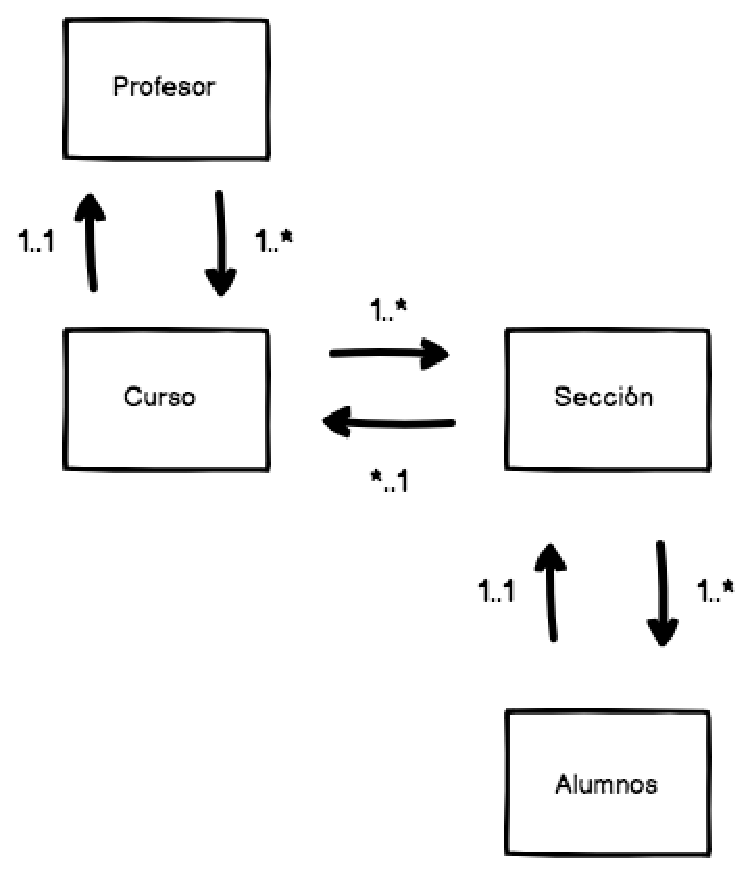
\includegraphics[width=0.3\textwidth]{img/base_de_datos.eps}
\end{figure}

\end{frame}
%++++++++++++++++++++++++++++++++++++++++++++++++++++++++++++++++++++++++++++++  

\subsection{Diseño de la aplicación}
%++++++++++++++++++++++++++++++++++++++++++++++++++++++++++++++++++++++++++++++  
\begin{frame}
\frametitle{Diseño de la aplicación}

La primera vez que se accede a la aplicación, el profesor, que será el que se registre en la aplicación, verá una descripción de en qué consiste la plataforma y lo que ofrece al profesorado
en los cursos impartidos.

\begin{figure}
    \includegraphics[width=0.5\textwidth]{img/captura_inicio.eps}
\end{figure}

\end{frame}
%++++++++++++++++++++++++++++++++++++++++++++++++++++++++++++++++++++++++++++++
\begin{frame}
\frametitle{Diseño de la aplicación}

El usuario tendrá tanto la posibilidad de crearse una cuenta y, en caso de estar registrado previamente, podrá iniciar sesión con la misma.

\begin{figure}[!th]%
    \centering
    \subfloat{{\includegraphics[width=4cm]{img/registro.eps} }}%
    \qquad
    \subfloat{{\includegraphics[width=4cm]{img/inicio_sesion.eps} }}%
\end{figure}

\end{frame}
%++++++++++++++++++++++++++++++++++++++++++++++++++++++++++++++++++++++++++++++
\begin{frame}
\frametitle{Diseño de la aplicación}

Una vez que el profesor haya accedido a la plataforma, tendrá a su disposición los cursos que ha creado previamente en forma de cuadrícula, con su información asociada.

\begin{figure}
    \includegraphics[width=0.6\textwidth]{img/cursos_creados.eps}
\end{figure}

\end{frame}
%++++++++++++++++++++++++++++++++++++++++++++++++++++++++++++++++++++++++++++++
\begin{frame}
\frametitle{Diseño de la aplicación}

Los detalles del curso, junto con las secciones impartidas del mismo, se pueden observar en los detalles del curso.

\begin{figure}
    \includegraphics[width=0.6\textwidth]{img/curso_secciones.eps}
\end{figure}

\end{frame}
%++++++++++++++++++++++++++++++++++++++++++++++++++++++++++++++++++++++++++++++
\begin{frame}
\frametitle{Diseño de la aplicación}

La representación gráfica de los resultados de los cursos/talleres estarán disponibles tanto para observarlos en la plataforma, como para descargar en formato PDF informe con los mismos.

\begin{figure}
    \includegraphics[width=0.6\textwidth]{img/estadisticas_seccion.eps}
\end{figure}

\end{frame}
%++++++++++++++++++++++++++++++++++++++++++++++++++++++++++++++++++++++++++++++


\section{Pruebas y verificación}
%++++++++++++++++++++++++++++++++++++++++++++++++++++++++++++++++++++++++++++++  
\begin{frame}
\frametitle{Pruebas y verificación}

Para llevar a cabo el ''\textit{testeo}'' de la plataforma, se usó RSpec, una herramienta utilizada con más frecuencia en el entorno de producción. Permite la verificación de diversas pruebas en modelos,
controladores, etc.

\begin{figure}[!th]%
    \centering
    \subfloat{{\includegraphics[width=5cm]{img/pruebas_curso.eps} }}%
    \qquad
    \subfloat{{\includegraphics[width=5cm]{img/pruebas_seccion.eps} }}%
\end{figure}

\end{frame}
%++++++++++++++++++++++++++++++++++++++++++++++++++++++++++++++++++++++++++++++
\begin{frame}
\frametitle{Pruebas y verificación}

\begin{exampleblock}{Tests}
    Se realizaron las pruebas sobre algunos de los \textbf{modelos} de la aplicación (Curso, Secciones y Usuarios), que se comprueba que se pasan con éxito, como se observa en la figura.
\end{exampleblock}

\begin{figure}
    \includegraphics[width=0.4\textwidth]{img/resultado_pruebas.eps}
\end{figure}

\end{frame}
%++++++++++++++++++++++++++++++++++++++++++++++++++++++++++++++++++++++++++++++


\section{Summary and conclusions}

%++++++++++++++++++++++++++++++++++++++++++++++++++++++++++++++++++++++++++++++  
\begin{frame}
\frametitle{Summary and conclusions}

\begin{ejemplo}
  \begin{enumerate}
    \item
    The developed platform, called CodeCharts, aims to make it easier for teachers to visualize the progress of their students, so that once the students have made the challenges, they can see if the courses or workshops are helping in the future promotioning computational thinking when facing activities.
      \pause
    \item
    One of the features of this application is that it is designed so that it is only used by the teaching staff, for that reason it has been developed for its use in the most simple and comfortable way.
  \end{enumerate}
\end{ejemplo}

\end{frame}
%++++++++++++++++++++++++++++++++++++++++++++++++++++++++++++++++++++++++++++++  

%++++++++++++++++++++++++++++++++++++++++++++++++++++++++++++++++++++++++++++++  
\begin{frame}[allowframebreaks]
  \frametitle{Bibliografía}

  \begin{thebibliography}{10}

    \beamertemplatebookbibitems
    \bibitem[URL: Code.org]{latex} 
    Code.org. {\small{\url{https://code.org/}}}

    \beamertemplatebookbibitems
    \bibitem[URL: Hour of Code]{latex} 
    Hour of Code. {\small{\url{https://hourofcode.com/}}}

    \beamertemplatebookbibitems
    \bibitem[URL: Codecademy]{latex} 
    Codecademy. {\small{\url{https://www.codecademy.com/es}}}

    \beamertemplatebookbibitems
    \bibitem[URL: Programamos]{latex} 
    Programamos. {\small{\url{https://programamos.es/}}}

    \beamertemplatebookbibitems
    \bibitem[URL: Ruby on Rails]{latex} 
    Ruby on Rails. {\small{\url{https://rubyonrails.org/}}}

    \beamertemplatebookbibitems
    \bibitem[URL: Active Record Basics]{latex} 
    Active Record Basics. {\small{\url{http://guides.rubyonrails.org/active_record_basics.html}}}

    \beamertemplatebookbibitems
    \bibitem[URL: Bootstrap]{latex} 
    Bootstrap. {\small{\url{https://getbootstrap.com/}}}

    \beamertemplatebookbibitems
    \bibitem[URL: Chartkick]{latex} 
    Chartkick. {\small{\url{https://www.chartkick.com/}}}

    \beamertemplatebookbibitems
    \bibitem[URL: Github]{latex} 
    Github. {\small{\url{https://github.com/}}}

    \beamertemplatebookbibitems
    \bibitem[URL: RSpec]{latex} 
    RSpec. {\small{\url{http://rspec.info/}}}

    \beamertemplatebookbibitems
    \bibitem[URL: PuntoQ]{latex} 
    PuntoQ. {\small{\url{http://www.bbtk.ull.es/view/institucional/bbtk/Biblioteca_Digital/es}}}

    \beamertemplatebookbibitems
    \bibitem[URL: ACM]{latex} 
    ACM. {\small{\url{https://www.acm.org/publications/magazines}}}

    \beamertemplatebookbibitems
    \bibitem[URL: IEEE]{latex} 
    IEEE. {\small{\url{https://www.ieee.org/publications/periodicals.html}}}

    \beamertemplatebookbibitems
    \bibitem[URL: SQLite]{latex} 
    SQLite. {\small{\url{https://rubygems.org/gems/sqlite3/versions/1.3.11?locale=es}}}

    \beamertemplatebookbibitems
    \bibitem[URL: Devise]{latex} 
    Devise. {\small{\url{https://rubygems.org/gems/devise}}}

    \beamertemplatebookbibitems
    \bibitem[URL: Gem Bootstrap]{latex} 
    Gem Bootstrap. {\small{\url{https://rubygems.org/gems/bootstrap}}}

    \beamertemplatebookbibitems
    \bibitem[URL: Will-paginate]{latex} 
    Will-paginate. {\small{\url{https://rubygems.org/gems/will_paginate}}}

    \beamertemplatebookbibitems
    \bibitem[URL: Wicked-PDF]{latex} 
    Wicked-PDF. {\small{\url{https://rubygems.org/gems/wicked_pdf}}}

    \beamertemplatebookbibitems
    \bibitem[URL: Jquery-Rails]{latex} 
    Jquery-Rails. {\small{\url{https://rubygems.org/gems/jquery-rails}}}

    \beamertemplatebookbibitems
    \bibitem[Wilson, Cameron]{beamer} 
    Wilson, Cameron. 
    \emph{Hour of Code: Bringing Research to Scale} 
    {\small{\url{http://doi.acm.org.accedys2.bbtk.ull.es/10.1145/2746406}}}

    \beamertemplatebookbibitems
    \bibitem[M. Wing]{beamer} 
    M. Wing. 
    \emph{COMMUNICATIONS OF THE ACM March} 
    {\small{\url{https://www.cs.cmu.edu/{~}CompThink/papers/Wing06.pdf}}}

    \beamertemplatebookbibitems
    \bibitem[Tumlin, Nath]{beamer} 
    Tumlin, Nath. 
    \emph{Teacher Configurable Coding Challenges for Block Languages} 
    {\small{\url{http://doi.acm.org.accedys2.bbtk.ull.es/10.1145/3017680.3022467}}}

    \beamertemplatebookbibitems
    \bibitem[Brown, Neil C.C. and Monig, Jens and Bau, Anthony and Weintrop, David]{beamer} 
    Brown, Neil C.C. and Monig, Jens and Bau, Anthony and Weintrop, David. 
    \emph{Panel: Future Directions of Block-based Programming} 
    {\small{\url{http://doi.acm.org.accedys2.bbtk.ull.es/10.1145/2839509.2844661}}}


  \end{thebibliography}
\end{frame}


%++++++++++++++++++++++++++++++++++++++++++++++++++++++++++++++++++++++++++++++  

\end{document}
